%!TEX root=paper.tex

\begin{abstract}

  Python is one of the fastest growing programming languages at the moment. Flask, a Python-based web framework is the technology used by tens of thousands of web applications. These applications, from interactive websites to service APIs, lack a technology-specific service monitoring solution. 

  In this paper, we present \tool, a tool that provides insight into the utilization and performance of evolving Flask-based web services. We present the ease with which the tool can be integrated in an already existing web application, discuss some of the visualization perspectives that the library provides, and point to some future challenges for similar libraries.

\end{abstract}




\section{Introduction}


% \todo{motivate with: monitoring in a world which is becoming more and more service-oriented is essential because it allows to perform three main types of actions: system adaptations to provide the request service at the desired level of quality, enabling flexibility in dealing with changing requirements and modes of operation, and enabling operational awareness through dashboards organizing the collected data~\cite{pernici2016monitoring}. In this work we focus on the last part and we discuss how a minimal effort probe-based solution for a particular type of web services can be used to facilitate the other two types of actions by involving the developer.}

% \todo{explain: in~\cite{vogel2017low} we introduced the \tool an a high level with a focus on presenting its performance visualization aspects; in this work we only summarize these features by means of introducing some of the provided functionalities of the \tool. We focus on discussing how the tool is implemented and operating, provide a deeper look at its capabilities for integration with version control and continuous integration environments, introduce a mechanism for performance prediction, and provide an evaluation of the proposed approach based on a case study. }

%Every system is a distributed system nowadays \cite{cavage2013there}. Indeed a very large number of applications and web applications are nowadays implemented as two-tier architectures with a front-end implemented with web technologies and a service back-end.
%\ml{I'm not completely happy with this paragraph}
{\em There is no getting around it: you are building a distributed system} argues Mark Cavage  in a recent article written for the {\em Communications of the ACM} \cite{cavage2013there}. Indeed, even the simplest second-year student project these days is a web application implemented as two-tier architecture with a Javascript/HTML5 front-end a service backend, usually a REST API.

% \hfill mds
% Many contemporary programming languages are offering libraries, modules, or frameworks that facilitate the development of such architectures. 
Python is one of the most popular programming language choices for implementing the back-end of web applications. GitHub contains more than 500K open source Python projects and the Tiobe Index\footnote{TIOBE programming community index is a measure of popularity of programming languages, created and maintained by the TIOBE Company based in Eindhoven, the Netherlands} ranks Python as the 4th most popular programming language as of June 2016. An analysis of  StackOverflow from September 2017 argues that {\em ``Python has a solid claim to being the fastest-growing major programming language''}\footnote{https://stackoverflow.blog/2017/09/06/incredible-growth-python/}.
 
% possible flask summary
Within the Python community, Flask\footnote{\url{http://flask.pocoo.org/}} is a very popular web framework\footnote{More than 25K projects on GitHub (5\% of all Python projects) are implemented with Flask (cf. a GitHub search for ``language:Python Flask'')}. It provides simplicity and flexibility by implementing a bare-minimum web server, and thus advertises as a micro-framework. The Flask tutorial shows how setting up a simple Flask {\em ``Hello World''} web-service requires no more than 5 lines of Python code \cite{ flask:tutorial}.
% end of summary
 
Despite their popularity however, and to the best of our knowledge, there is no simple solution for monitoring the evolving performance of Flask web applications. Thus, every one of the developers of these projects faces one of the following options when confronted with the need of gathering insight into the runtime behavior of their implemented services: 

  \begin{enumerate}

    \item Use a commercial monitoring tool which treats the subject API as a black-box (e.g. Pingdom, Runscope). 
    % , Graphite+Graphana+statd etc.

    \item Implement their own ad-hoc analytics solution, having to reinvent basic visualization and interaction strategies. 

    \item Live without analytics insight into their services.

  \end{enumerate}

%\todo{For the first point in the list, we can also argue that analytics solutions like Google Analytics can be used, but they have no notion of versioning/integration with the development life cycle. Feel free to cite \cite{papazoglou2011managing} for service evolution purposes}

For projects on a budget (e.g. research, startups) the first and the second options are often not available due to time and financial constraints. Even when using 3rd-party analytics solutions, a critical insight into the evolution of the exposed services of the web application is missing because such solutions have no notion of versioning and no integration with the development life cycle~\cite{papazoglou2011managing}.

To avoid projects ending up in the third situation, that of living without analytics, in this paper we present \tool~ --- a low-effort service monitoring library for Flask-based Python web services that is easy to integrate and enables the {\em agile assessment} of service evolution~\cite{Nier12b}. 

As a case study, on which we will illustrate our solution, we are going to use an open source API which, for several years, was in the third of the above-presented situations, i.e. it was being operated without any monitoring solution.

% In the next section, we will present a case study of an open source research API which was for a long time in the third situation presented above -- deployed without analytics insight.

\subsection*{Extending Previous Work}

This paper is an extension of [Anonymous Paper by Anonymous Auhthors] which was published as a NIER paper in [Anonymous Conference]. The current paper extends that paper in the following ways: 
\begin{itemize}
  \item Providing more details about the case study in Section \ref{sec:case} and extending the data collection period by half a year.
  \item New perspectives and a better categorization of the perspectives are presented in Sections \ref{sec:utilandperf} -- \ref{sec:evolution}.
  \item A detailed discussion on automated outlier detection and monitoring is provided (Section \ref{sec:outliers}).
  \item An advanced discussion on the integration with continuous integration environments in order to triangulate the live collected data with information from testing the endpoints with a constant load and introduce a mechanism for performance prediction is added (Section \ref{sec:testing})
  \item A more extended discussion about lessons learned while developing the tool including measurements on the overhead incurred by the presented tool (Sections \ref{sec:overhead} and \ref{sec:discussion})
\end{itemize}



\section{Case Study}

% \subsection{An Ecosystem With a Service API at its Core}
\label{sec:api}
\label{sec:case}

  \zee
  % \footnote{\url{https://github.com/zeeguu-ecosystem/}} 
  is a platform and an ecosystem of applications for accelerating vocabulary acquisition in a foreign language \cite{lungu18-chi}. 
%
  The architecture of the ecosystem has at its core an API and a series of ecosystem applications that together offer to a learner three main inter-dependent features:

  \begin{enumerate}

    \item \textit{Reader applications} that provide one-click (or one touch, on touch-enabled devices) translations for the words and expressions in a text that the reader does not understand. Besides facilitating reading, the translations serve as input to a user knowledge model that is used further to generate personalized exercises and further reading recommendations.

    \item \textit{Interactive exercises} are generated based on the texts that the reader has studied in the past and are scheduled in such a way as to optimize the memory retention and to prioritize the most important unknown vocabulary items.

    \item \textit{Article recommendations} are also personalized for the interests and language capabilities of each learner. The recommendations come with a difficulty estimation that helps the learner find articles with appropriate difficulty.

  \end{enumerate}

  \Fref{fig:zeeguuarch} presents a high-level view of the case study ecosystem.  The core API is implemented with Flask and Python and provides three types of functionality, respectively: contextual translations, personalized exercise suggestions, and article recommendations. In total, the API provides a bit under 50 endpoints in total, out of which around a dozen are very frequently used. The development of the core API itself is a research project. 
  % One of the authors of this paper is part of the developer team that maintains and evolves the \zee API. 


    \begin{figure}[h!]
      \centering
      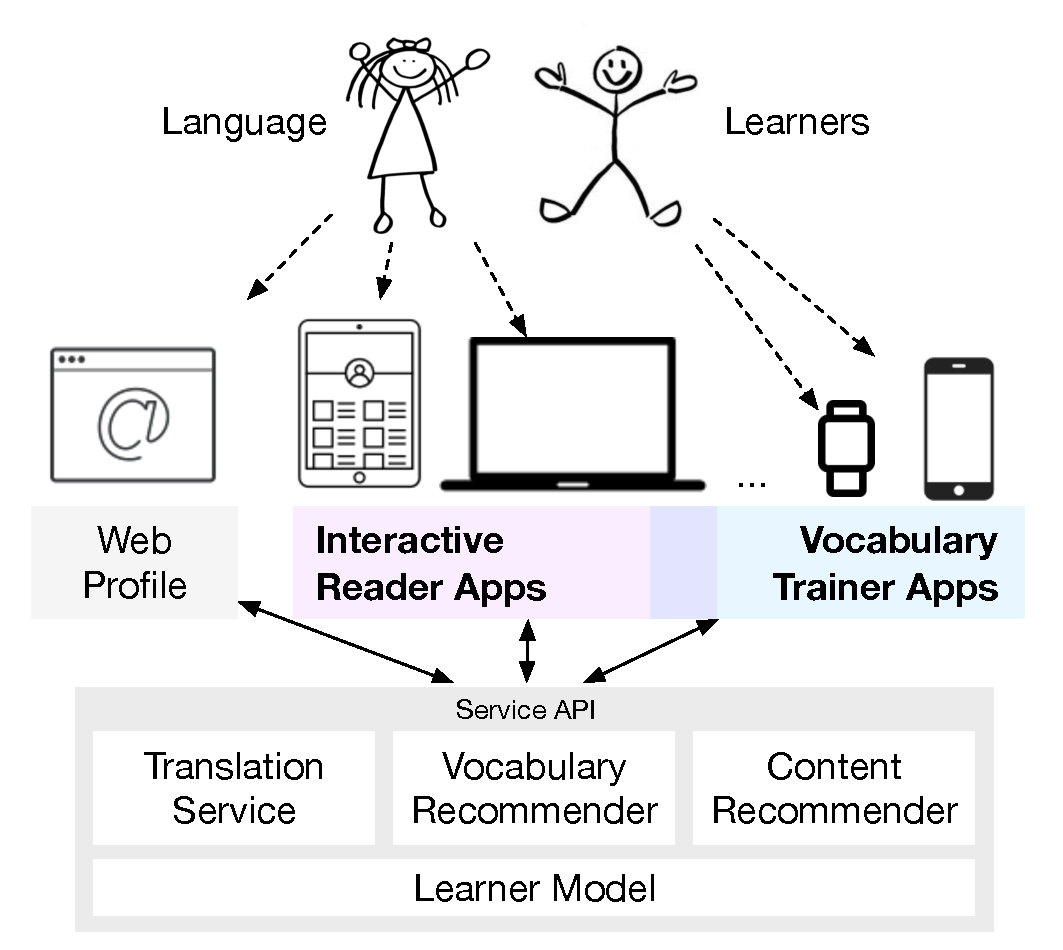
\includegraphics[width=0.7\linewidth]{zeeguu-architecture}
      \caption{The architecture of the \zee ecosystem \cite{lungu18-chi}}
      \label{fig:zeeguuarch}
    \end{figure}  


  At the time of writing, the ecosystem consists of a reader web application, a web-based exercises platform, and a smartwatch application, which are used by more than \activeUserCount active users on a regular basis. The users come from several Dutch highschools and a language center associated with a Dutch University. Several users are using it on their own, outside of any formal educational context. The learners use \zee to study a variety of foreign languages including German, Dutch, and French. They have also diverse native languages, including: Chinese, Dutch, and English. The system can scale to many languages by delegating the machine translation tasks to third party APIs. 



\subsection{Study characteristics}

  We will use this \zee service API as a case study for this paper. It is open source, and has been deployed for several years without any monitoring
  solution until June 2017, when the \tool has been deployed with it. 
  During the ten month deployment (between June 2017 and the time of writing this
  article, April 2018) more than 112.000 requests
  to the API have been recorded by the API \footnote{Note that the 
  recorded requests are a lower bound on the usage of the API, 
  as only a subset of the API endpoints have been actually instrumented} . The highest load observed 
  until now on the API consisted of 12K requests in a single day. 
  With the help of the applications in the ecoystem, in the aforementioned
  time period the users have 
  performed about 30K vocabulary exercises and have translated 
  about 28K words and experssions while reading foreign language 
  texts. 

  All the figures and measurements in this paper are captured from the actual deployment of \tool in the context of the \zee API. The figures are interactively offering basic data exploration capabilities: filter, zoom, and details on demand~\cite{Shne99a}. The \tool deployment for the case study can be accessed publicly\footnote{\url{https://zeeguu.unibe.ch/api/dashboard}; username: {\em guest}, password: {\em icsme}}. 


 % \todo{create new account, update URL if necessary, update activeUserCount, add a couple of sentences of the current state of the case study with the college/language center}
% \ml{we should consider adding also one section in which the architecture/implementation and main features of the dashboard are presented before going on with discussing them in more depth in the following sections --- this should include a rundown on which views are provided from where (overview or per endpoint)}



\subsection{The Technology Stack}
\label{sec:flask}

 As discussed in the previous section, Flask is a microframework for Python. 
 The ``micro'' in microframework means Flask aims to keep the core simple but extensible. 
 The framework does not make many decisions for the user, such as what database to use and
 those decisions that it does make, such as what templating engine to use, can be changed. 

 Flask is built on top of WSGI\footnote{\url{http://wsgi.org}} --- The Web Server Gateway Interface --- a calling convention for web servers to forward requests to web applications or frameworks written in Python. A Python web application based on WSGI has to have one central callable object that implements the actual application. In Flask this is an instance of the Flask class. Each Flask application has to create an instance of this class itself and pass it the name of the module. The following code snippet presents a simple ``Hello World'' web service written in Python with the help of the Flask framework. 

\begin{lstlisting}[style=custompython]

from flask import Flask
app = Flask(__name__)

@app.route('/')
def index():
    return 'Hello World!'

\end{lstlisting}

In the following we discuss the capabilities of the \tool in more depth.



